% !TEX program = xelatex
\documentclass[]{article}
\usepackage{commons/course}

\begin{document}
\printheader

\section*{سوال اول}
\subsection*{قسمت الف}
یکی از کار‌هایی که می‌توان کرد این است یک تبادل کلید دیفی هلمن انجام گیرد به صورتی که تمامی
پارامتر‌ها با کلید
$K_{c,s}$
امضا شوند. (مثلا به کمک الگوریتم \lr{CBC-MAC}) با این کار تنها
$C$ و $V$
و
$KDC$
می‌توانند که پارامتر‌ها را امضا کنند و از انجا که
$KDC$
نمی‌تواند ترافیکی را عوض کند می‌دانیم که حمله‌ی مرد میانی نمی‌تواند رخ دهد و کلید جدید
$K'$
صرفا بین دو
$C$ و $V$
ساخته می‌شود و فقط این دو کلید را دارند.
\subsection*{قسمت ب}
همان طور که در قسمت قبل هم گفته شد در این صورت حمله مرد میانی می‌تواند صورت بگیرد چرا که خود
$KDC$
می‌تواند که پارامتر‌ها را امضا بکند.
\subsection*{قسمت پ}
به نظر من یکی از کار‌های نسبتا ساده‌ای که می‌توان انجام داد این است که یکی از طرفین کلید تصادفی
$K'$
را تولید کند و سپس آن را در ابتدا با
$K_{c,s,1}$ و در ادامه با $K_{c,s,2}$
رمز می‌کند. در این حالت در صورتی که
$KDC1$
بخواهد که رمز را باز کند نیاز دارد که کلید
$KDC2$
را بداند و در صورتی که
$KDC2$
بخواهد رمز را باز کند باید کلید
$KDC1$
را بداند. از انجا که فرض کردیم تبانی نداریم پس این کار را نمی‌توانند انجام دهند.
در نهایت نیز برای صحت ارسال می‌توان هم با
$K_{c,s,1}$ و هم $K_{c,s,2}$
کلید را امضا کرد و سپس آن را رمز کرد.
\section*{سوال دوم}
\subsection*{قسمت الف}
برای ساخت کلید من از
\link{https://irtfweb.ifa.hawaii.edu/~lockhart/gpg/}{این}
لینک استفاده کردم. همان طور که مشخص است در ابتدا از دستور
\LRE{\verb|gpg --gen-key|}
استفاده می‌کنیم. در ادامه تمامی موارد خواسته شده را وارد می‌کنیم و یک پسورد برای کلید خود انتخاب می‌کنیم.
نتیجه دستور در شکل
\ref{fig:gpg:keygen}
موجود است.
\begin{figure}[H]
    \centering
    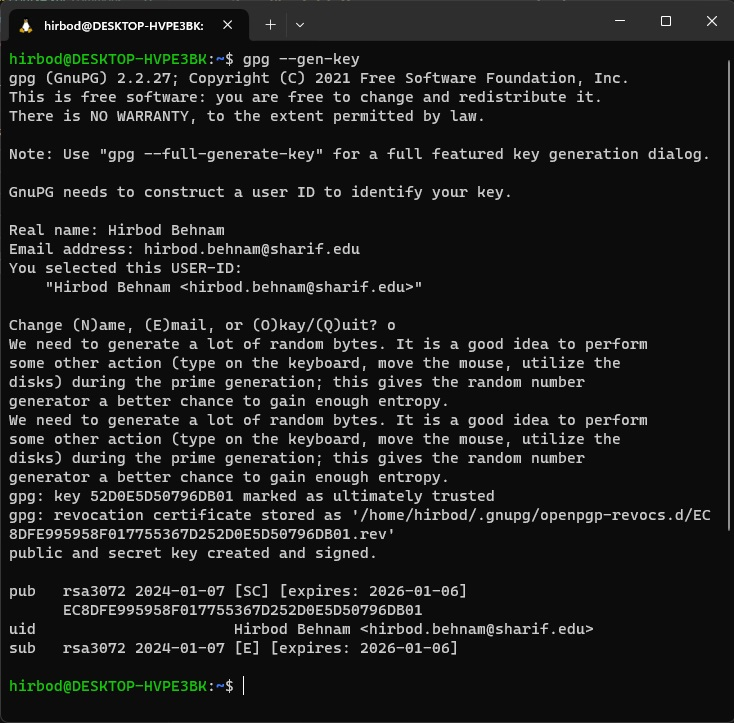
\includegraphics[scale=0.75]{pics/gpg-keygen.jpg}
    \caption{ساخت \lr{GPG key}}
    \label{fig:gpg:keygen}
\end{figure}
حال می‌توانیم با دستور
\LRE{\verb|gpg --list|}
تمامی کلید‌های خود را مشاهده کنیم. همچنین می‌توان با دستور زیر کلید عمومی مربوط به دانشگاه را استخراج کرد.
\begin{latin}
\begin{lstlisting}[language=sh]
gpg --export -a "hirbod.behnam@sharif.edu"
\end{lstlisting}
\end{latin}
نتیجه این دستورات را می‌توانید در شکل
\ref{fig:gpg:view}
ببینید.
\begin{figure}[H]
    \centering
    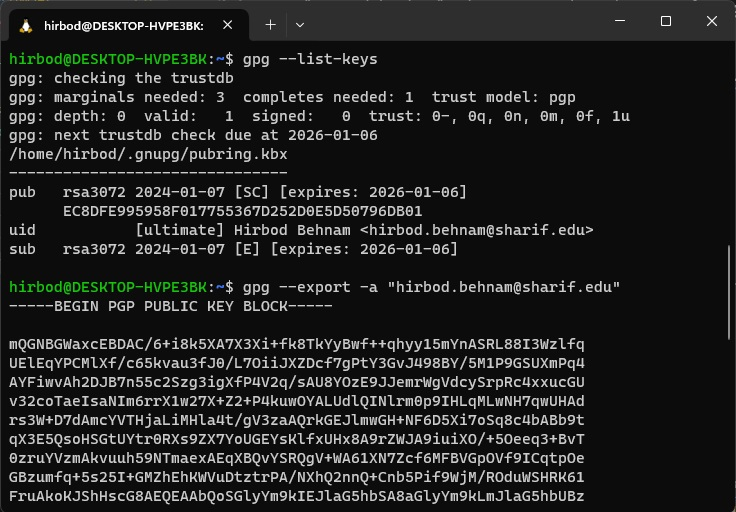
\includegraphics[scale=0.5]{pics/gpg-view.jpg}
    \caption{مشاهده کلید‌های PGP}
    \label{fig:gpg:view}
\end{figure}
\subsection*{قسمت ب}
در این قسمت در ابتدا نیاز است که کلید عمومی داده شده را
import
کنیم. برای این کار از دستور زیر استفاده می‌کنیم. نتیجه‌ی آن در عکس
\ref{fig:gpg:import}
آمده است.
\begin{latin}
\begin{lstlisting}[language=sh]
gpg --import Reza_0xCFBEEE88_public.asc
\end{lstlisting}
\end{latin}
\begin{figure}[H]
    \centering
    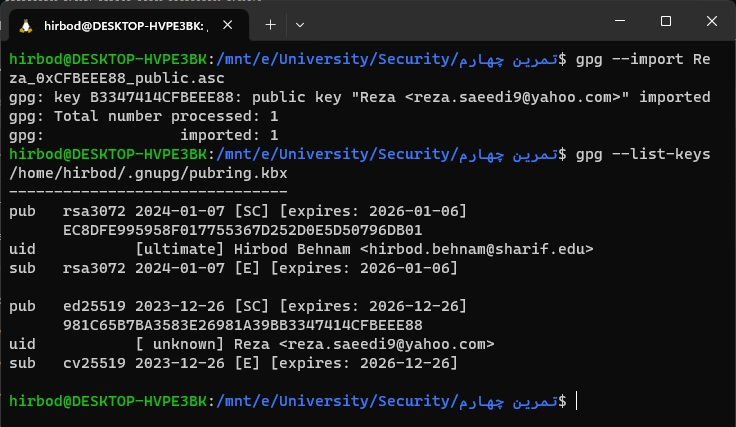
\includegraphics[scale=0.5]{pics/gpg-import.jpg}
    \caption{اضافه کردن کلید PGP طراح تمرین به GPG}
    \label{fig:gpg:import}
\end{figure}
حال باید دیتایی را در ابتدا امضا و سپس رمزنگاری کنیم. برای این کار از دستور زیر استفاده می‌کنیم.
دقت کنید که این دستور یک فایل را رمزنگاری و امضا می‌کند. در نتیجه کافی است که صرفا متن ایمیل را در فایلی
بنویسیم و آن فایل را رمز کنیم.
(\link{https://medium.com/@acparas/how-to-encrypt-and-sign-a-file-with-gpg-531070b2fa6d}{منبع})
\begin{latin}
\begin{lstlisting}[language=sh]
gpg --output email.pgp --armor --encrypt --sign --recipient reza.saeedi9@yahoo.com email-plaintext.txt
\end{lstlisting}
\end{latin}
همان طور که مشاهده می‌کنید محتوای فایل تولید شده رمزگذاری شده است.
\begin{figure}[H]
    \centering
    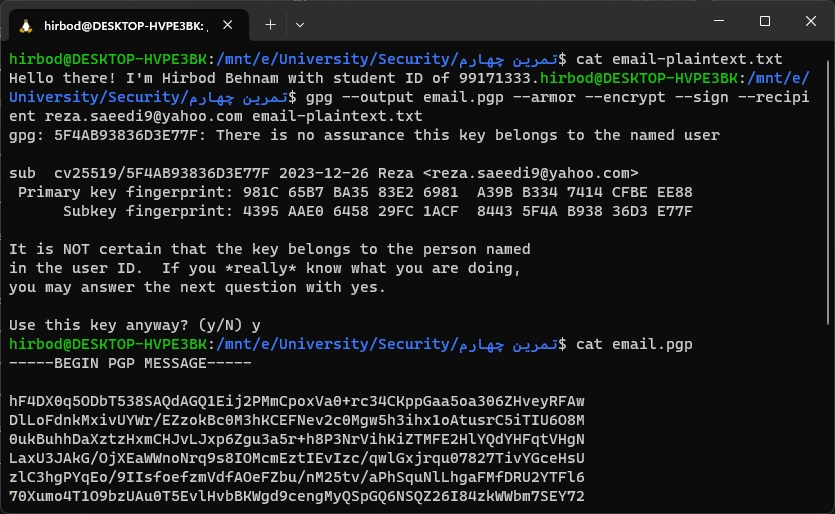
\includegraphics[scale=0.5]{pics/gpg-encrypt.jpg}
    \caption{رمزنگاری پیام}
    \label{fig:gpg:encrypt}
\end{figure}
در نهایت نیز محتوای این فایل را ایمیل کردم. دقت کنید که در کل مراحل بالا
\LRE{\verb|--armor|}
برای این بود که نتیجه به صورت اسکی کد باشد و بتوان آن را کپی و پیست در ایمیل کرد.
ایمیل فرستاده شده نیز در شکل
\ref{fig:gpg:email}
قابل مشاهده است.
\begin{figure}[H]
    \centering
    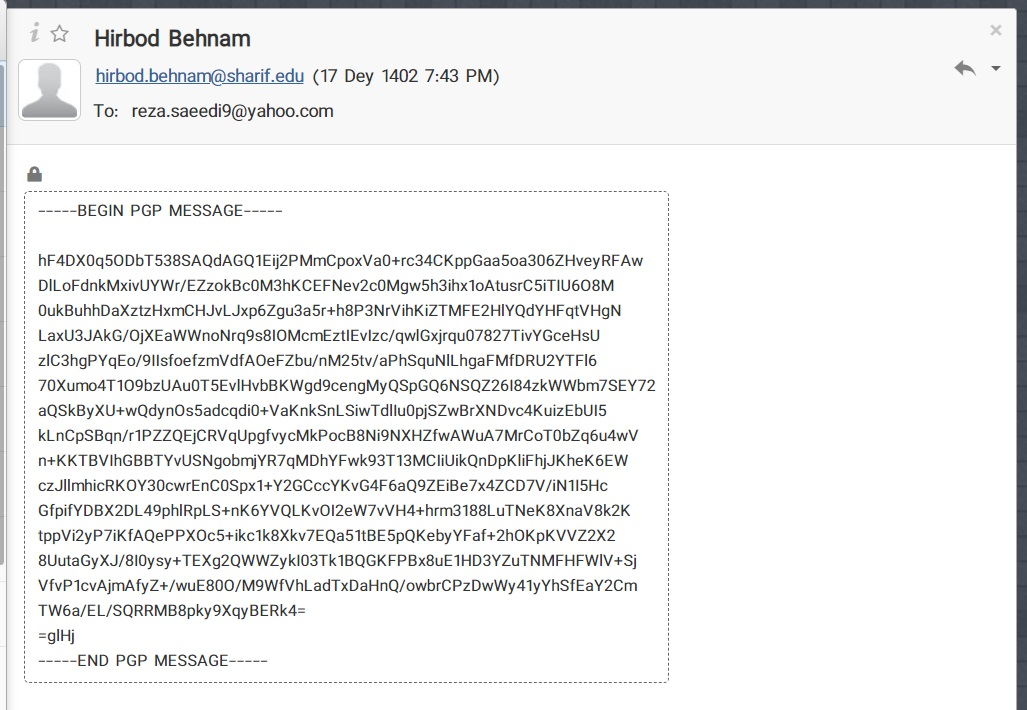
\includegraphics[scale=0.35]{pics/gpg-email.jpg}
    \caption{ایمیل فرستاده شده}
    \label{fig:gpg:email}
\end{figure}
\section*{سوال سوم}
\subsection*{قسمت الف}
\begin{itemize}
    \item \textbf{\lr{Bruteforce Attack}}: این حمله عملا سعی می‌کند که با حدس زدن کلید رمزنگاری رمزنگاری را بشکاند. به صورت صریح این مورد در درس ذکر نشده است اما من فکر می‌کنم که به صورت کلی نمی‌توان جلوی \lr{bruteforce} را گرفت اما می‌توان احتمال آن را کم کرد. به عنوان مثال می‌توان از الگوریتم‌های رمزنگاری قوی استفاده کرد.
    \item \textbf{\lr{Known Plaintext Attack}}: در این حمله مهاجم هم یک متن به صورت رمزگشایی شده را دارد و هم یک متن به صورت رمزشده را دارد. این نوع حمله نیز به کمک \lr{cipher} استفاده شده می‌تواند بی اثر شود.
    \item \textbf{\lr{Reply Attack}}: این حمله بدین صورت است که مهاجم یکی از پکت‌های قبلی کاربر را بدون تغییر به سرور می‌فرستد. این حمله به کمک استفاده از \lr{sequence number} و \lr{window} قابل جلوگیری است چرا که پیام‌هایی که در قبل دریافت شده‌اند را داریم و در صورت مشاهده‌ی یک پیام تکراری آن را دور می‌ریزیم.
    \item \textbf{\lr{Password Sniffing}}: این حمله زمانی اتفاق می‌افتد که مثلا رمز یک سایت را به صورت \lr{plaintext} برای سرور ارسال کنیم و افرادی که به کانکشن ما گوش می‌کنند می‌توانند آن را ببنیند و ضبط کنند. اما \lr{IPSec} کار که می‌کند در مدل ESP این است که تمامی داده‌ها را رمز می‌کند پس دیگر نمی‌توان پسورد‌ها را بدست آورد.
    \item \textbf{\lr{IP Spoofing}}: این حمله بدین صورت است که پکت‌هایی درست می‌کنیم که IP مبدا را عوض می‌کنیم و چیزی به غیر از آی‌پی واقعی خود قرار می‌دهیم. (\link{https://en.wikipedia.org/wiki/IP_address_spoofing}{منبع}) این مورد به کمک امضا‌هایی که در الگوریتم اتفاق می‌افتد خنثی می‌شود چرا که فرستند به کمک \lr{IP} خودش یک امضا می‌زند. پس اگر کسی دیگر بخواهد که \lr{IP} را عوض کند امضا را نیز باید بتواند عوض کند.
    \item \textbf{\lr{IP Hijacking}}: این نوع حملات بدین صورت هستند که واقعا \lr{IP}هایی را در شبکه در اختیار می‌گیریم که برای ما نیست و دیتا‌هایی که برای ما نباید بیاید برای ما می‌آید.  (\link{https://www.oreilly.com/library/view/hackers-beware/0735710090/0735710090_ch05lev1sec1.html}{منبع}) نوع مقابله با این حمله نیز مانند قسمت قبل است. البته دقت کنید که اگر کامل \lr{redicet} صورت بگیرد فرد دیگر نمی‌تواند پکت‌ها را باز کند چرا که کلید‌ها را ندارد.
    \item \textbf{\lr{SYN Flooding}}: در این نوع حمله یک مهجام یک عالمه پکت \lr{SYN} که اولین پکت برای شروع یک کانکشن TCP است را برای یک سرور به تعداد زیادی می‌فرستد به طوری که IP مبدا آن برای شخص دیگر باشد. (\link{https://www.cloudflare.com/learning/ddos/syn-flood-ddos-attack/}{منبع}) اما نکته‌ای که وجود دارد این است که IPSec صرفا اصالت و محرمانگی را برای ما تامین می‌کند. پس جلوی این حمله را نمی‌تواند بگیرد. (\link{https://security.stackexchange.com/a/177035}{منبع})
\end{itemize}
\subsection*{قسمت ب}
در این قسمت من از دو ماشین مجازی
\lr{Ubuntu 22.04}
استفاده کردم که به یک اداپتور
\lr{host only}
در
\lr{Virtualbox}
وصل بودند. با این کار می‌توان که از هر کدام از ماشین مجازی‌ها دیگری را پینگ کرد. اولین ماشین مجازی بروی روی
\lr{192.168.207.4} است و دیگری بر روی \lr{192.168.207.5}
است. در ادامه از آموزش در
\link{https://www.gypthecat.com/ipsec-vpn-host-to-host-on-ubuntu-14-04-with-strongswan}{این لینک}
استفاده می‌کنیم. در ابتدا باید
\lr{strongswan}
را نصب کنیم. برای این کار در
\lr{Ubuntu}های
نسخه‌های جدید از دستور زیر استفاده می‌کنیم.
(\link{https://www.linode.com/docs/guides/strongswan-vpn-server-install/}{منبع})
\begin{latin}
\begin{lstlisting}[language=sh]
apt install strongswan strongswan-pki libcharon-extra-plugins libcharon-extauth-plugins libstrongswan-extra-plugins libtss2-tcti-tabrmd0
\end{lstlisting}
\end{latin}
سپس فایل
\LRE{\verb|/etc/ipsec.conf|}
را ویرایش می‌کنیم و محتوای آن را در ماشین مجازی با آی‌پی
\lr{192.168.207.4}
برابر زیر قرار می‌دهیم:
\begin{latin}
\begin{lstlisting}[language=sh]
config setup

conn first-server
    authby=secret
    auto=route
    keyexchange=ike
    left=192.168.207.4
    right=192.168.207.5
    type=transport
    esp=aes128gcm16!
\end{lstlisting}
\end{latin}
همچنین در فایل
\LRE{\verb|/etc/ipsec.secrets|}
مقدار زیر را قرار می‌دهیم:
\begin{latin}
\begin{lstlisting}[language=sh]
192.168.207.4 192.168.207.5 : PSK "My Password"
\end{lstlisting}
\end{latin}
حال دو دستور زیر را اجرا می‌کنیم و نتیجه آن‌ها را بررسی می‌کنیم.
\begin{latin}
\begin{lstlisting}[language=sh]
ipsec restart
ipsec statusall
\end{lstlisting}
\end{latin}
\begin{figure}[H]
    \centering
    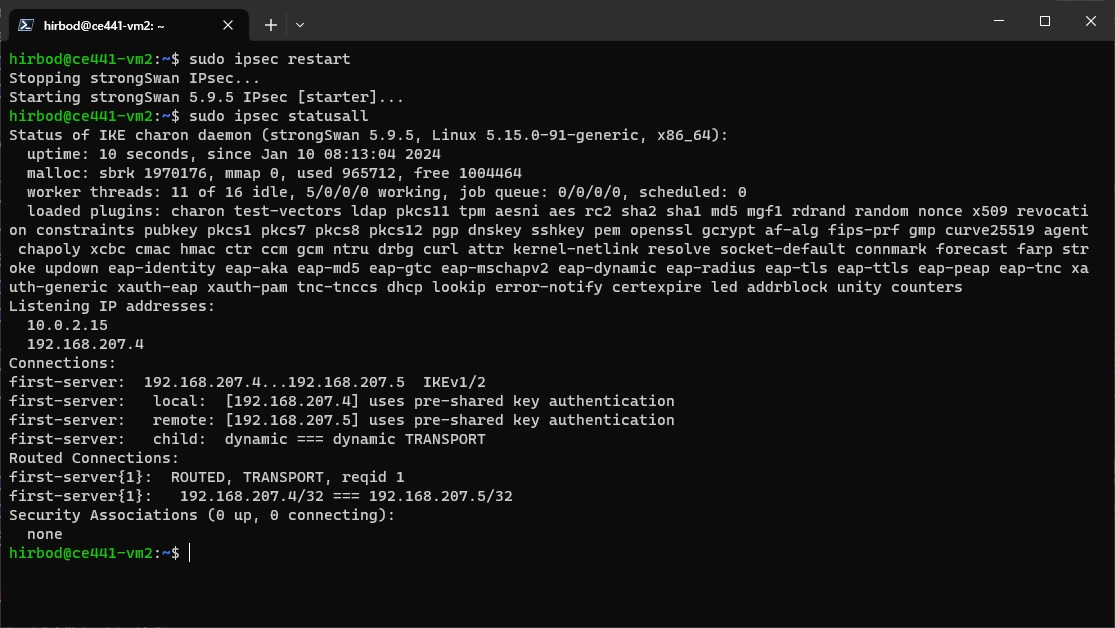
\includegraphics[scale=0.5]{pics/ipsec-stat1.jpg}
    \caption{وضعیت strongswan در سرور اول}
\end{figure}
حال برای سرور دوم نیز همین کارها را انجام می‌دهیم با این تفاوت که جای آی‌پی‌ها را عوض می‌کنیم.
یعنی فایل
\LRE{\verb|/etc/ipsec.conf|}
به صورت زیر است:
\begin{latin}
\begin{lstlisting}[language=sh]
config setup

conn second-server
    authby=secret
    auto=route
    keyexchange=ike
    left=192.168.207.5
    right=192.168.207.4
    type=transport
    esp=aes128gcm16!
\end{lstlisting}
\end{latin}
و فایل
\LRE{\verb|/etc/ipsec.secrets|}
به صورت زیر:
\begin{latin}
\begin{lstlisting}[language=sh]
192.168.207.5 192.168.207.4 : PSK "My Password"
\end{lstlisting}
\end{latin}
در نهایت نیز دو دستور آخر را اجرا می‌کنیم:
\begin{figure}[H]
    \centering
    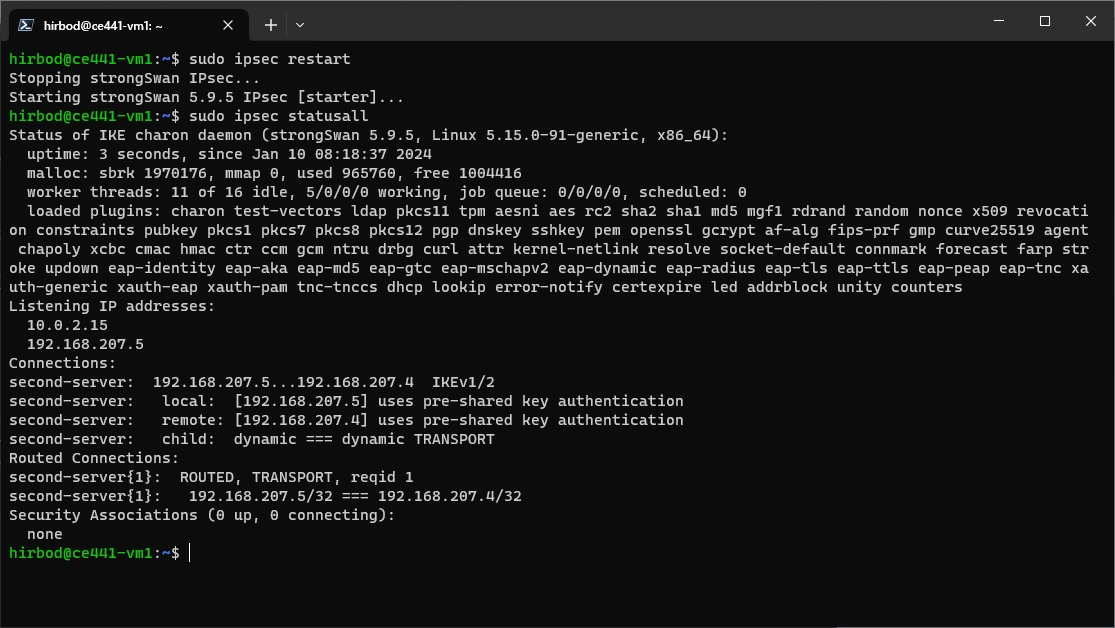
\includegraphics[scale=0.5]{pics/ipsec-stat2.jpg}
    \caption{وضعیت strongswan در سرور دوم}
\end{figure}
حال از یکی از سرور‌ها دیگری را پینگ می‌کنیم و وضعیت
\lr{IPSec}
را چک می‌کنیم. همان طور که مشاهده می‌کنید تعداد پکت‌های دریافتی زیاد می‌شود.
\begin{figure}[H]
    \centering
    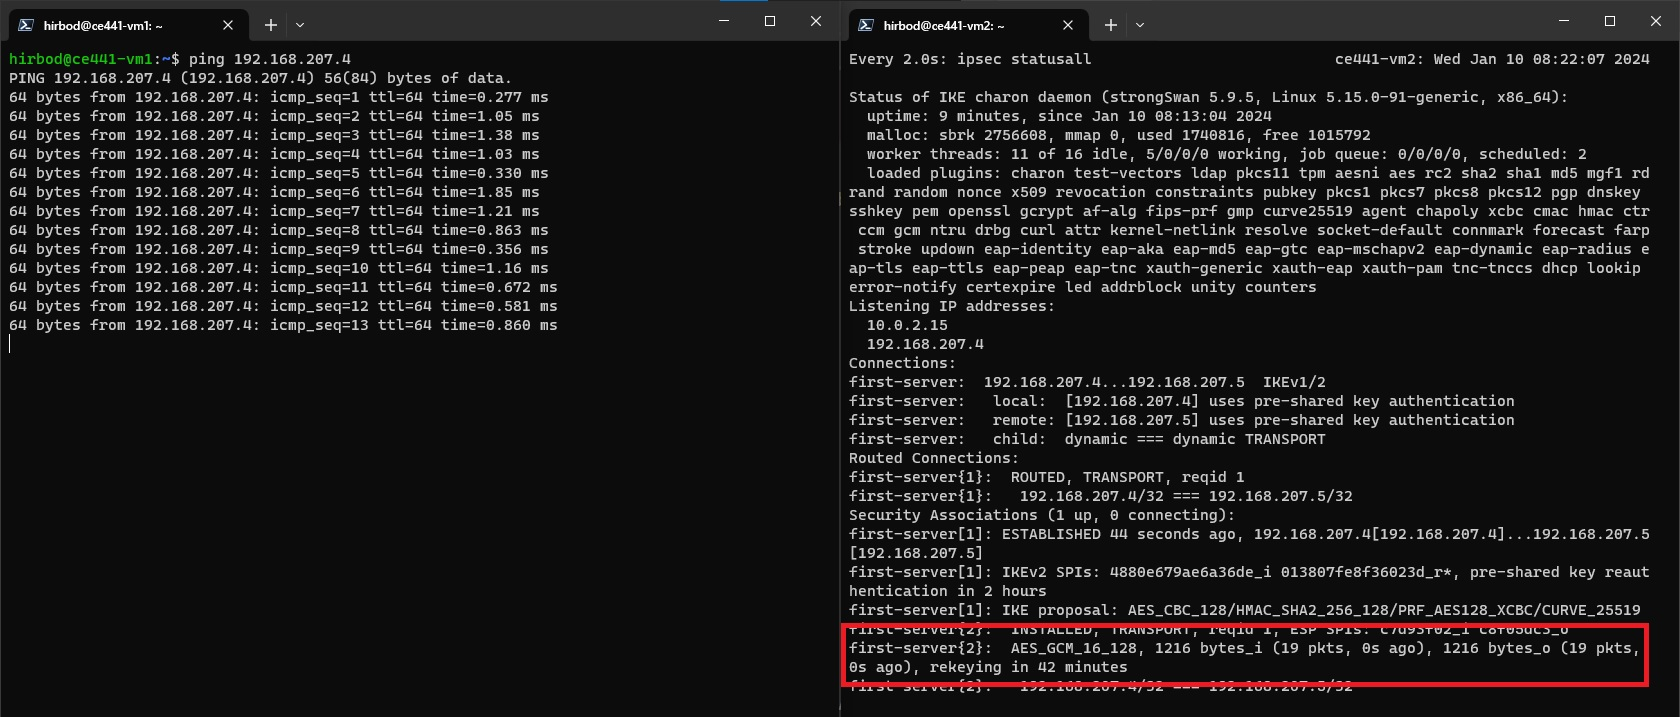
\includegraphics[scale=0.32]{pics/ipsec-ping.jpg}
    \caption{پینگ کردن از یک سرور به سرور دیگر}
\end{figure}
همچنین در نهایت نیز پکت‌ها را به کمک
\lr{tcpdump}
بررسی می‌کنیم. برای این کار از دستور زیر استفاده می‌کنیم که پکت‌هایی که از آن یکی
\lr{VM}
می‌آید را
\lr{capture}
کنیم.
\begin{latin}
\begin{lstlisting}[language=sh]
tcpdump -i enp0s8 src 192.168.207.5 -w ipsec.pcap
\end{lstlisting}
\end{latin}
سپس فایل
\verb|ipsec.pcap|
را با
\lr{wireshark}
باز می‌کنیم.
\begin{figure}[H]
    \centering
    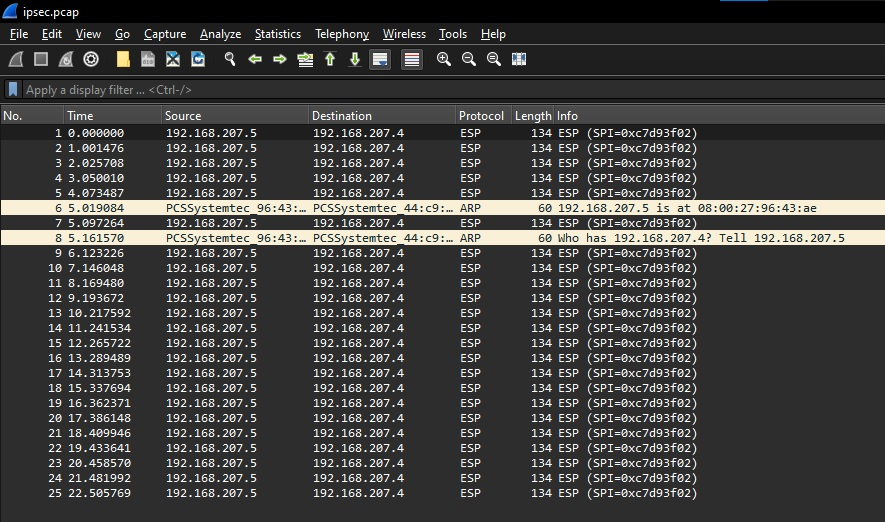
\includegraphics[scale=0.6]{pics/ipsec-pcap.jpg}
    \caption{مشاهده پکت‌های \lr{ipsec} در \lr{wireshark}}
\end{figure}
فایل
\verb|ipsec.pcap|
نیز به تمرین پیوست شده است.
\section*{سوال چهارم}
در ابتدا برای استفاده از
\lr{TLS 1.2}
من از دستور زیر در
\lr{curl}
استفاده کردم چرا که به نظر سوال برای \lr{TLS 1.2}
طراحی شده است و اکثرا سایت‌ها در حال حاضر از
\lr{TLS 1.3}
استفاده می‌کنند.
(\link{https://superuser.com/a/976171}{منبع})
\begin{latin}
\begin{lstlisting}[language=sh]
curl --tlsv1.2 --tls-max 1.2 https://google.com
\end{lstlisting}
\end{latin}
سپس به کمک
\lr{wireshark}
پکت‌های رد و بدل شده را بررسی کردم. فایل فیلتر شده پکت‌ها نیز به تمرین پیوست شده است.
\subsection*{قسمت الف}
به ترتیب پکت‌ها و محتوای آن در زیر آمده است»
\begin{enumerate}
    \item از کامپیوتر من به سرور می‌رود و شامل \lr{Client Hello} است.
    \item این پکت از سرور به کلاینت می‌آید و شامل \lr{Server Hello} است.
    \item این پکت نیز از سرور به کلاینت می‌آید و شامل سه \lr{record} است. یکی از آنها شامل \lr{certificate} است، بعدی شامل \lr{server key exchange} است که پارامتر‌های دیفی هلمن فرستاده می‌شود و آخری \lr{server hello done} است.
    \item این پکت از کامپیوتر من به سرور می‌رود و شامل سه \lr{record} است. یکی برای پارامتر‌های دیفی هلمن، دیگری برای \lr{change cipher spec} که بگویید به سرور که رمزنگاری شروع شود و آخری برای \lr{encrypted handshake message} که نشان دهیم که رمزگذاری می‌تواند انجام شود.
    \item این پکت نیز از سرور به کلاینت می‌آید که سه \lr{record} دارد. اولی برای \lr{new session ticket} است که یک نشست جدید را مشخص می‌کند، دیگری برای \lr{change cipher spec} که بگویید به کلاینت که رمزنگاری شروع شود و آخری برای \lr{encrypted handshake message} که نشان دهیم که رمزگذاری می‌تواند انجام شود.
    \item این پکت رمز شده از کلاینت به سرور می‌رود و احتمالا حاوی هدرهای HTTP است. اسم این پروتکل \lr{Application Data Protocol} است.
    \item این بسته از سرور به کلاینت می‌رود و احتمالا حاوی هدر‌های HTTP جواب است.
    \item این پکت نیز مانند پکت قبل است.
\end{enumerate}
در ادامه هر رکورد سه فیلد ثابت دارد.
\begin{enumerate}
    \item \textbf{\lr{Content Type}}: یک بایت است و مشخص می‌کند که این چه رکوردی است.
    \item \textbf{\lr{Version}}: ورژن TLS است که دو بایت است و یک بایت برای major و دیگری برای minor است.
    \item \textbf{\lr{Length}}: طول محتوای بسته که دو بایت است.
\end{enumerate}
\subsection*{قسمت ب}
در پکت اول
\lr{content type} برابر ۲۲ یا \lr{Handshake} است.
همچنین من حدس میزنم که در
\lr{wireshark}
مقدار
\lr{nonce}
همان فیلد
\lr{Random}
است. این فیلد در
\lr{server hello}
باید عینا بیاید و برای همین می‌توان تشخیص داد که
\lr{replay attack}
اتفاق نیفتاده است.
(\link{https://security.stackexchange.com/a/157710}{منبع})
همچنین
\lr{cipher suite}های
من در شکل زیر آمده است:
\begin{figure}[h]
    \centering
    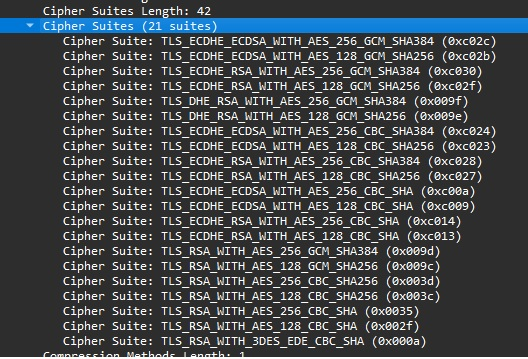
\includegraphics[scale=0.5]{pics/tls-ciphers.jpg}
    \caption{تمامی \lr{cipher suite}های این handshake}
\end{figure}
\subsection*{قسمت پ}
در کانکشن من \lr{cipher suite} برابر
\lr{TLS ECDHE ECDSA WITH AES 128 GCM SHA256}
است که از الگوریتم
\lr{AES} ۱۲۸ بیتی استفاده می‌کند.
همان طور که در قسمت قبل گفتم
\lr{client random}
عینا فرستاده می‌شود.
\lr{Session ID}
به ما این قابلیت را می‌دهد که یک
\lr{Session}
قبلی را ادامه دهد. یعنی تمامی الگوریتم و کلید‌ها و غیره همان قبلی هستد.
(\link{https://security.stackexchange.com/a/190497}{منبع})
در اینجا
\lr{certificate}
در رکورد و پکت دیگری فرستاده شده است.

برای
\lr{certificate}
همان طور که در عکس زیر مشخص است کلید عمومی با الگوریتم
\lr{secp256r1}
است و طول کلید آن با توجه به اسم الگوریتم ۲۵۶ بیت است. خود
\lr{certificate}
نیز با الگوریتم
\lr{RSA} و چکیده ساز \lr{SHA256}
امضا شده است. خود گواهی نیز از طرف
\lr{Google Trust Services LLC}
امضا شده است.
\begin{figure}[h]
    \centering
    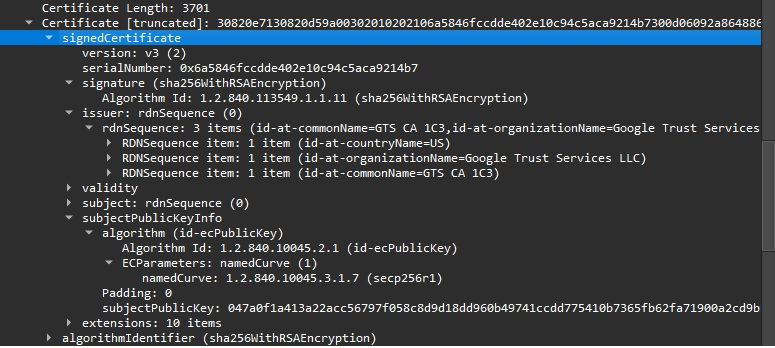
\includegraphics[scale=0.5]{pics/tls-cert.jpg}
    \caption{مقادیر مربوط به \lr{certificate}}
\end{figure}
\subsection*{قسمت ت}
برای من همچین فیلدی وجود ندارد!
\begin{figure}[h]
    \centering
    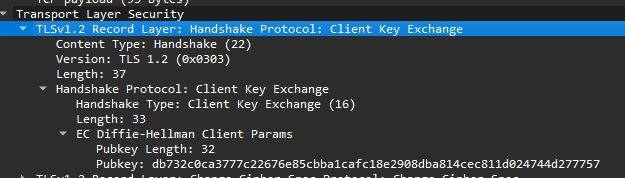
\includegraphics[scale=0.5]{pics/tls-client-key-exchange.jpg}
    \caption{پکت \lr{client key exchange}}
\end{figure}
اما من در
\link{https://tls12.xargs.org/}{این سایت}
نگاه کردم و دیدم که به نظر می‌آید که این یک فیلد نیست بلکه یک عملیات است که بر روی کلید عمومی
سرور و کلید خصوصی خود کلاینت انجام می‌شود و باعث می‌شود که سرور و کلاینت به یک کلید مشترک برسند مثل دیفی هلمن.
سپس با این کلید در رکورد‌های
\lr{client handshake finished} و \lr{server handshake finished}
هش تمامی پکت‌های قبلی حساب می‌شود و رمز می‌شود و همچنین مهم تر از آن کلید‌های رمزگذاری و مک زدن و غیره به کمک آن تولید می‌شود.
\subsection*{قسمت ث}
خیر فرقی ندارد و صرفا به طرف مقابل می‌گوید که می‌توانیم پیام‌های رمزشده را شروع کنیم. پکت
\lr{Encrypted Handshake}
نیز برای فرستادن یک پیام رمزشده به سرور یا کلاینت استفاده می‌شود که طرف مقابل مطمئن باشد که
رمزنگاری درست انجام شده است.
\subsection*{قسمت ج}
به کمک کلید‌هایی که در قبل رد و بدل کردیم و الگوریتم‌هایی که توافق کردیم.
\section*{سوال پنجم}
\begin{enumerate}
    \item \link{https://superuser.com/a/634471}{منبع} \begin{latin}
\begin{lstlisting}[language=sh]
iptables -A OUTPUT -j ACCEPT
\end{lstlisting}
    \end{latin}
    \item \link{https://www.digitalocean.com/community/tutorials/iptables-essentials-common-firewall-rules-and-commands\#allowing-established-and-related-incoming-connections}{منبع 1} \link{https://www.ipserverone.info/knowledge-base/how-to-open-ports-in-iptables}{منبع 2} \begin{latin}
\begin{lstlisting}[language=sh]
iptables -A INPUT -j DROP
iptables -A INPUT -m conntrack --ctstate ESTABLISHED -j ACCEPT
iptables -I INPUT -p tcp --dport 22 -j ACCEPT
\end{lstlisting}
\end{latin}
    \item \link{https://www.cyberciti.biz/tips/linux-iptables-9-allow-icmp-ping.html}{منبع} \begin{latin}
\begin{lstlisting}[language=sh]
iptables -A INPUT -p icmp -j ACCEPT
iptables -A INPUT -p icmp --icmp-type redirect -j DROP
\end{lstlisting}
    \end{latin}
    \item برای این قسمت در ابتدا باید قابلیت \lr{IP forwarding} را در لینوکس فعال کنیم. برای این کار کافی است که از دستور زیر استفاده کنیم: \begin{latin}
\begin{lstlisting}[language=sh]
echo "net.ipv4.ip_forward=1" >> /etc/sysctl.conf
\end{lstlisting}
\end{latin}
    سپس در ادامه باید دستگاه را یک بار ری استارت کنیم. در نهایت نیز از دستورات زیر استفاده می‌کنیم: \link{https://unix.stackexchange.com/a/585613}{منبع}
\begin{latin}
\begin{lstlisting}[language=sh]
iptables -t nat -A PREROUTING -p tcp --dport 8080 -j DNAT --to-destination 127.0.0.1:80
iptables -t nat -A POSTROUTING -j MASQUERADE
\end{lstlisting}
\end{latin}
    \item برای این سوال من در گوگل صرفا سرچ کردم که چه قوانینی برای iptables و مقابله با DDOS خوب هستند که به
    \link{https://gist.github.com/mattia-beta/bd5b1c68e3d51db933181d8a3dc0ba64}{این لینک}
    رسیدم. از بین دستوراتی که در این لینک موجود بود برخی از آن‌ها که به نظرم تاثیرات خیلی خوب می‌توانست بگذارد را
    برداشتم و آن‌ها را در ادامه لیست کردم.
\begin{latin}
\begin{lstlisting}[language=sh]
# Drop invalid packets
iptables -t mangle -A PREROUTING -m conntrack --ctstate INVALID -j DROP
   
# Drop TCP packets that are new and are not SYN
/sbin/iptables -t mangle -A PREROUTING -p tcp ! --syn -m conntrack --ctstate NEW -j DROP

# Block packets with bogus TCP flags
iptables -t mangle -A PREROUTING -p tcp --tcp-flags FIN,SYN,RST,PSH,ACK,URG NONE -j DROP
iptables -t mangle -A PREROUTING -p tcp --tcp-flags FIN,SYN FIN,SYN -j DROP
iptables -t mangle -A PREROUTING -p tcp --tcp-flags SYN,RST SYN,RST -j DROP
iptables -t mangle -A PREROUTING -p tcp --tcp-flags SYN,FIN SYN,FIN -j DROP
iptables -t mangle -A PREROUTING -p tcp --tcp-flags FIN,RST FIN,RST -j DROP
iptables -t mangle -A PREROUTING -p tcp --tcp-flags FIN,ACK FIN -j DROP
iptables -t mangle -A PREROUTING -p tcp --tcp-flags ACK,URG URG -j DROP
iptables -t mangle -A PREROUTING -p tcp --tcp-flags ACK,FIN FIN -j DROP
iptables -t mangle -A PREROUTING -p tcp --tcp-flags ACK,PSH PSH -j DROP
iptables -t mangle -A PREROUTING -p tcp --tcp-flags ALL ALL -j DROP
iptables -t mangle -A PREROUTING -p tcp --tcp-flags ALL NONE -j DROP
iptables -t mangle -A PREROUTING -p tcp --tcp-flags ALL FIN,PSH,URG -j DROP
iptables -t mangle -A PREROUTING -p tcp --tcp-flags ALL SYN,FIN,PSH,URG -j DROP
iptables -t mangle -A PREROUTING -p tcp --tcp-flags ALL SYN,RST,ACK,FIN,URG -j DROP

# Limit connections per source IP
iptables -A INPUT -p tcp -m connlimit --connlimit-above 111 -j REJECT --reject-with tcp-reset

# Limit new TCP connections per second per source IP
iptables -A INPUT -p tcp -m conntrack --ctstate NEW -m limit --limit 60/s --limit-burst 20 -j ACCEPT
iptables -A INPUT -p tcp -m conntrack --ctstate NEW -j DROP
\end{lstlisting}
\end{latin}
    کاری که این دستورات می‌کنند این است که در ابتدا پکت‌هایی که اصلا شکل درستی ندارند (یعنی هیچ پروتکل \lr{TCP-UDP-ICMP}) نیستند
    را دراپ می‌کنیم. در ادامه جلوی پکت‌های TCP را می‌گیریم که به هیچ کانکشنی در سیستم‌عامل مپ نشده‌اند. بدین معنا که مثلا ممکن است مهاجمی
    یک پکت FIN برای یک کانکشنی بفرستد که وجود ندارد.
    در ادامه جلوی پکت‌های TCP را می‌گیریم که فلگ‌های آن‌ها ممکن نیست که حالت‌های خاصی داشته باشند. به عنوان مثال
    هیچ گاه یک پکت نمی‌توان SYN و FIN همزمان داشته باشد!
    در آخر که به نظر من مهم ترین کاری است که می‌توان انجام داد این است که تعداد کانکشن‌های TCP
    از یک IP را محدود کنیم. در اینجا به کاربران با یک IP اجزاه داده نمی‌شود که همزمان 111 و یا بیشتر کانکشن باز داشته باشند.
    در نهایت نیز سرعت باز کردن کانشکن‌های جدید را محدود می‌کنیم.
\end{enumerate}
\end{document}
